%
% ---------------------------------------------------------------
% Copyright (C) 2012-2018 Gang Li
% ---------------------------------------------------------------
%
% This work is the default powerdot-tuliplab style test file and may be
% distributed and/or modified under the conditions of the LaTeX Project Public
% License, either version 1.3 of this license or (at your option) any later
% version. The latest version of this license is in
% http://www.latex-project.org/lppl.txt and version 1.3 or later is part of all
% distributions of LaTeX version 2003/12/01 or later.
%
% This work has the LPPL maintenance status "maintained".
%
% This Current Maintainer of this work is Gang Li.
%
%

\documentclass[
 size=14pt,
 paper=smartboard,  %a4paper, smartboard, screen
 mode=present, 		%present, handout, print
 display=slides, 	% slidesnotes, notes, slides
 style=tuliplab,  	% TULIP Lab style
 pauseslide,
 fleqn,leqno]{powerdot}


%我自己增加的两端对其用
\usepackage{ragged2e}
\renewcommand{\raggedright}{\leftskip=0pt \rightskip=0pt plus 0cm}


\usepackage{cancel}
\usepackage{caption}
\usepackage{stackengine}
\usepackage{smartdiagram}
\usepackage{attrib}
\usepackage{amssymb}
\usepackage{amsmath} 
\usepackage{amsthm} 
\usepackage{mathtools}
\usepackage{rotating}
\usepackage{graphicx}
\usepackage{boxedminipage}
\usepackage{rotate}
\usepackage{calc}
\usepackage[absolute]{textpos}
\usepackage{psfrag,overpic}
\usepackage{fouriernc}
\usepackage{pstricks,pst-3d,pst-grad,pstricks-add,pst-text,pst-node,pst-tree}
\usepackage{moreverb,epsfig,subfigure}
\usepackage{color}
\usepackage{booktabs}
\usepackage{etex}
\usepackage{breqn}
\usepackage{multirow}
\usepackage{natbib}
\usepackage{bibentry}
\usepackage{gitinfo2}
\usepackage{siunitx}
\usepackage{nicefrac}
%\usepackage{geometry}
%\geometry{verbose,letterpaper}
\usepackage{media9}
\usepackage{animate}
%\usepackage{movie15}
\usepackage{auto-pst-pdf}

%\usepackage{breakurl}
\usepackage{fontawesome}
\usepackage{xcolor}
\usepackage{multicol}



\usepackage{verbatim}
\usepackage[utf8]{inputenc}
\usepackage{dtk-logos}
\usepackage{tikz}
\usepackage{adigraph}
%\usepackage{tkz-graph}
\usepackage{hyperref}
%\usepackage{ulem}
\usepackage{pgfplots}
\usepackage{verbatim}
\usepackage{fontawesome}


\usepackage{todonotes}
% \usepackage{pst-rel-points}
\usepackage{animate}
\usepackage{fontawesome}

\usepackage{listings}
\lstset{frameround=fttt,
frame=trBL,
stringstyle=\ttfamily,
backgroundcolor=\color{yellow!20},
basicstyle=\footnotesize\ttfamily}
\lstnewenvironment{code}{
\lstset{frame=single,escapeinside=`',
backgroundcolor=\color{yellow!20},
basicstyle=\footnotesize\ttfamily}
}{}


\usepackage{hyperref}
\hypersetup{ % TODO: PDF meta Data
  pdftitle={Kaggle sildes},
  pdfauthor={Wang Mingxi},
  pdfpagemode={FullScreen},
  pdfborder={0 0 0}
}


% \usepackage{auto-pst-pdf}
% package to show source code

\definecolor{LightGray}{rgb}{0.9,0.9,0.9}
\newlength{\pixel}\setlength\pixel{0.000714285714\slidewidth}
\setlength{\TPHorizModule}{\slidewidth}
\setlength{\TPVertModule}{\slideheight}
\newcommand\highlight[1]{\fbox{#1}}
\newcommand\icite[1]{{\footnotesize [#1]}}

\newcommand\twotonebox[2]{\fcolorbox{pdcolor2}{pdcolor2}
{#1\vphantom{#2}}\fcolorbox{pdcolor2}{white}{#2\vphantom{#1}}}
\newcommand\twotoneboxo[2]{\fcolorbox{pdcolor2}{pdcolor2}
{#1}\fcolorbox{pdcolor2}{white}{#2}}
\newcommand\vpspace[1]{\vphantom{\vspace{#1}}}
\newcommand\hpspace[1]{\hphantom{\hspace{#1}}}
\newcommand\COMMENT[1]{}

\newcommand\placepos[3]{\hbox to\z@{\kern#1
        \raisebox{-#2}[\z@][\z@]{#3}\hss}\ignorespaces}

\renewcommand{\baselinestretch}{1.2}


\newcommand{\draftnote}[3]{
	\todo[author=#2,color=#1!30,size=\footnotesize]{\textsf{#3}}	}
% TODO: add yourself here:
%
\newcommand{\gangli}[1]{\draftnote{blue}{GLi:}{#1}}
\newcommand{\shaoni}[1]{\draftnote{green}{sn:}{#1}}
\newcommand{\gliMarker}
	{\todo[author=GLi,size=\tiny,inline,color=blue!40]
	{Gang Li has worked up to here.}}
\newcommand{\snMarker}
	{\todo[author=Sn,size=\tiny,inline,color=green!40]
	{Shaoni has worked up to here.}}

%%%%%%%%%%%%%%%%%%%%%%%%%%%%%%%%%%%%%%%%%%%%%%%%%%%%%%%%%%%%%%%%%%%%%%%%
% title
% TODO: Customize to your Own Title, Name, Address
%
\title{The First Report}
\author{
Wang Mingxi
\\
\\Jilin University
\\College of Computer Science and Technology
}
\date{\gitCommitterDate}
%\date{\today} %暂时手写改动

% Customize the setting of slides
\pdsetup{
% TODO: Customize the left footer, and right footer
rf=\href{http://www.tulip.org.au}{
Last Changed by: \textsc{\gitCommitterName}\ \gitVtagn-\gitAbbrevHash\ (\gitAuthorDate)
%Last Changed by: \textsc{Mingxi Wang}\ \gitVtagn-\gitAbbrevHash\ (\today)
},
cf={FLIP01},
}


\begin{document}

\maketitle

%\begin{slide}{Overview}
%\tableofcontents[content=sections]
%\end{slide}


%	\begin{center}
%	\begin{figure}[htbp]
%		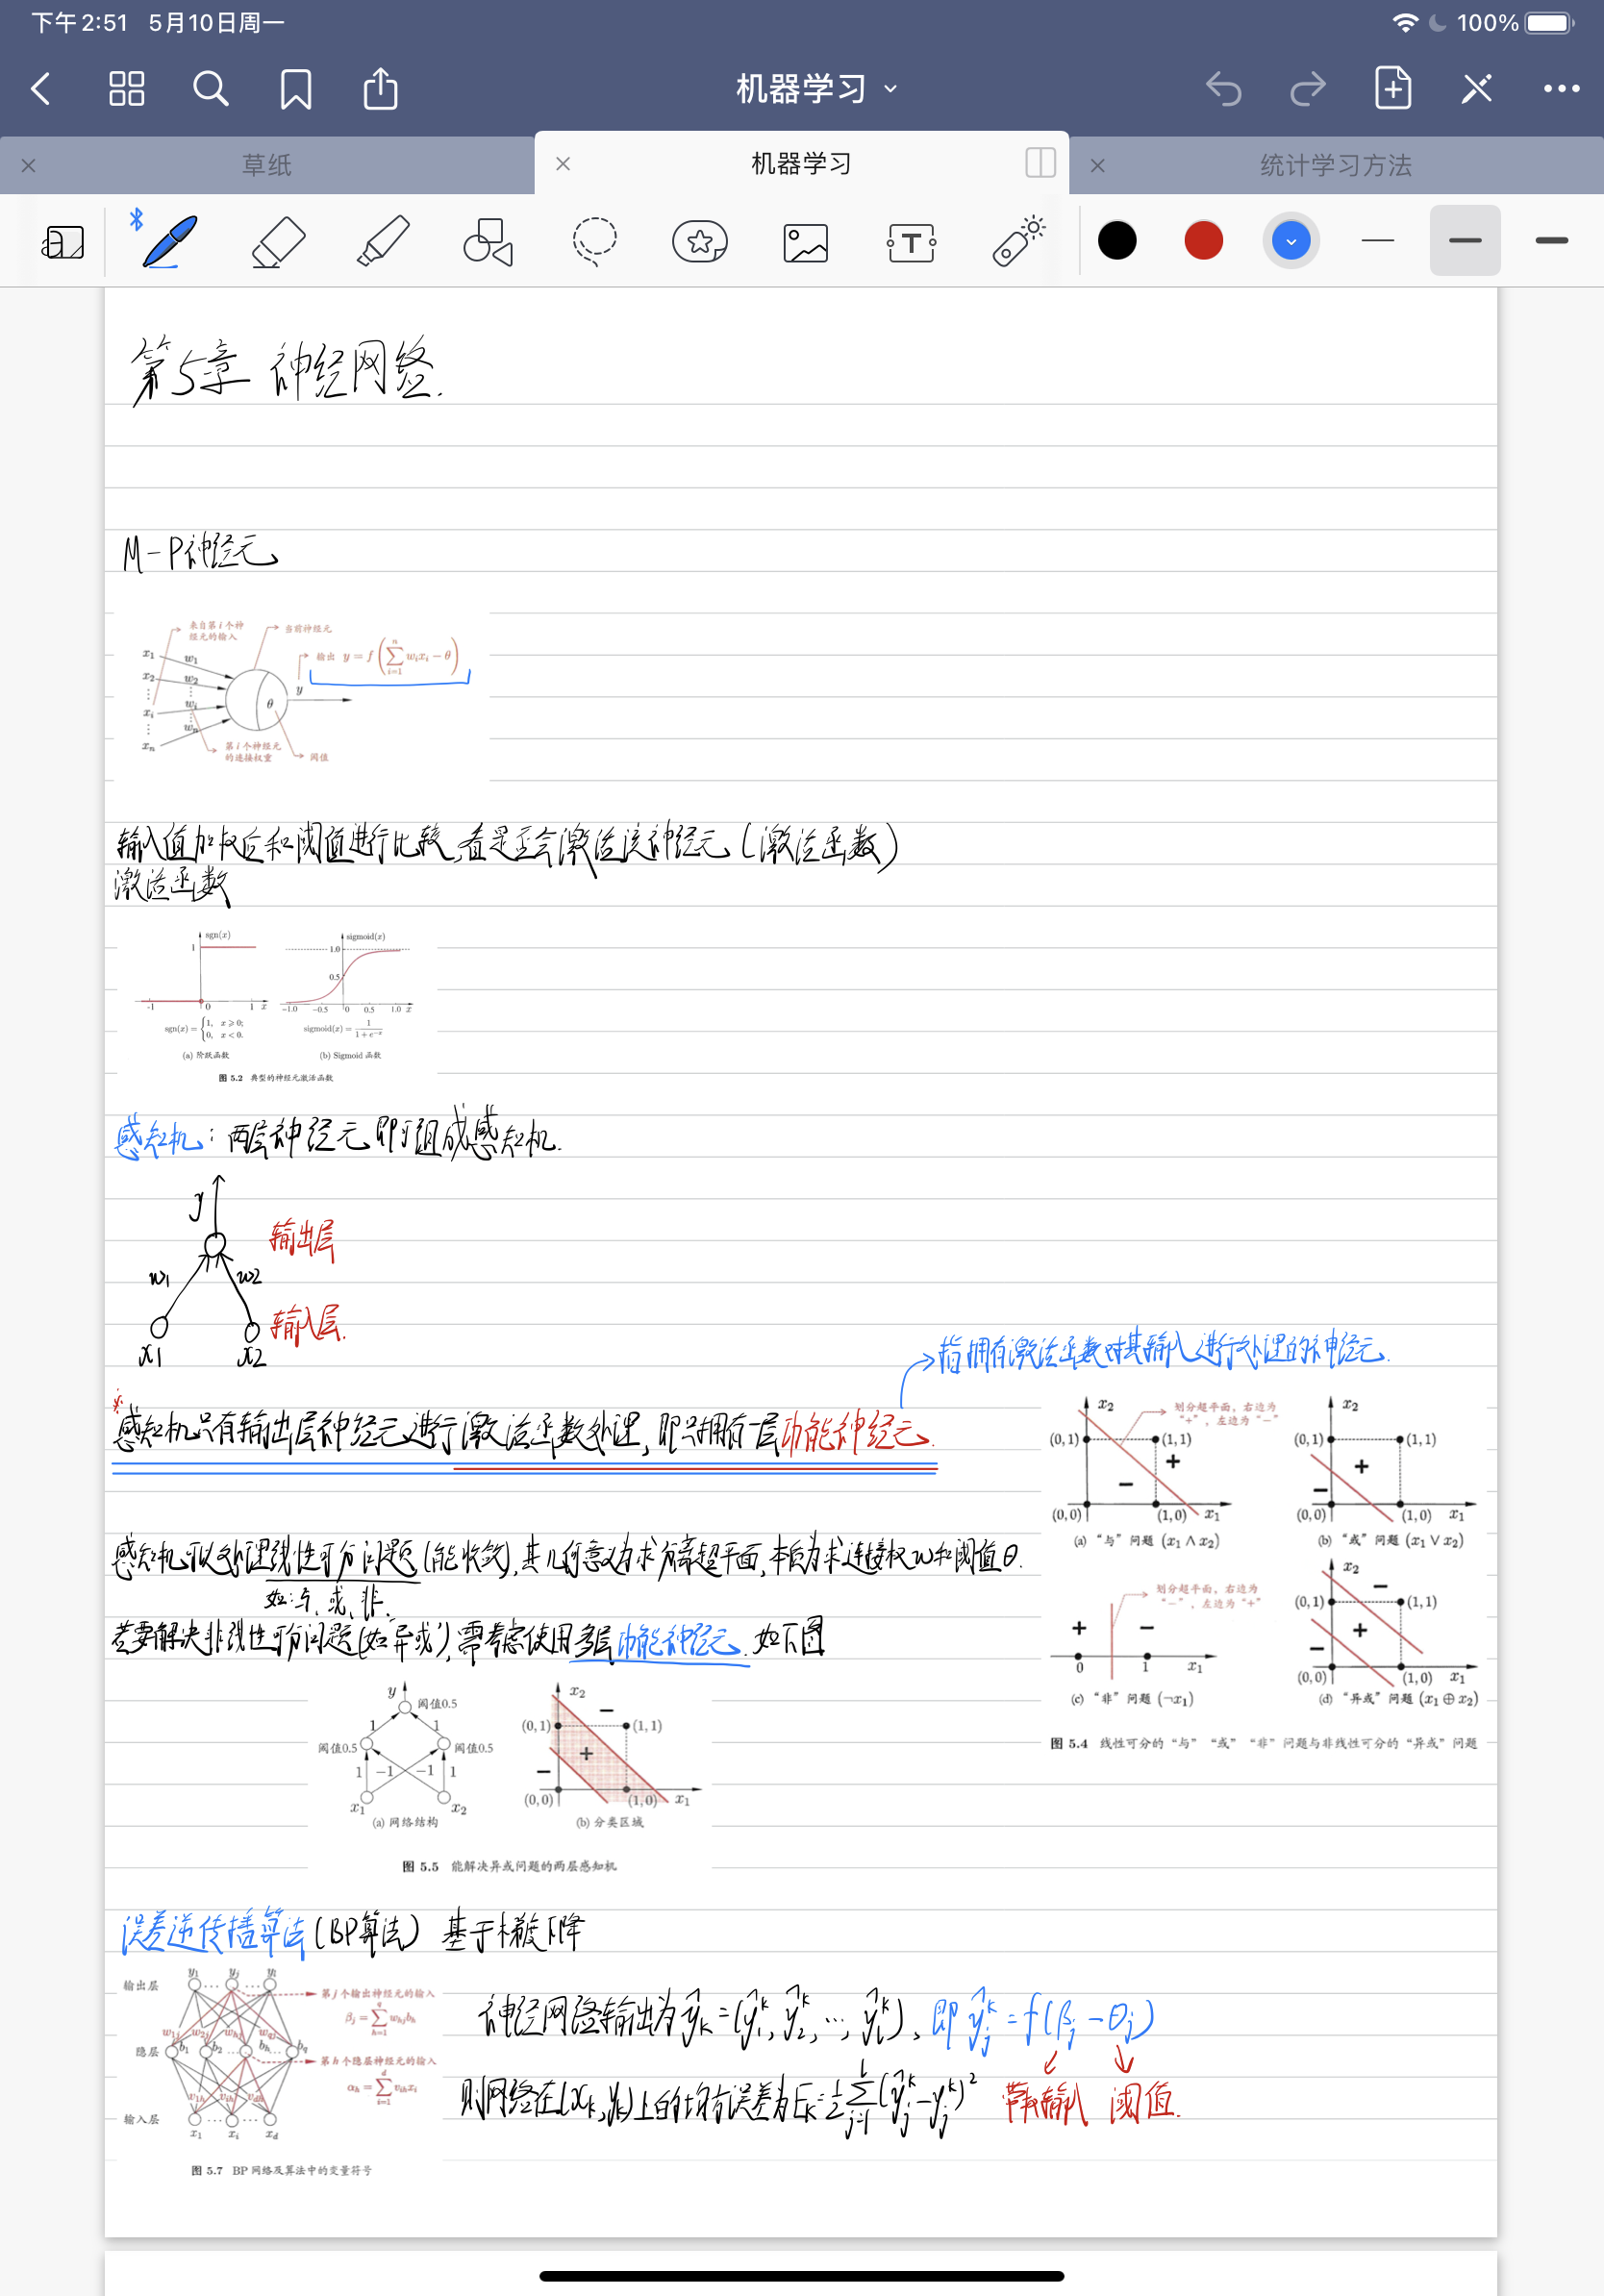
\includegraphics[scale=0.1]{./pic/11.eps}
%		\caption{project preview}
%	\end{figure}
%\end{center}


%%==========================================================================================
%%
\begin{slide}[toc=,bm=]{Overview}
\tableofcontents[content=currentsection,type=1]
\end{slide}
%%
%%==========================================================================================


\section{Learning content}

%%==========================================================================================
%%
\begin{slide}{Decision tree}
 Decision tree:A decision tree is a prediction model used to predict the category of samples.In the structure of these trees, leaf nodes give categories and inner nodes represent attributes.
 		\begin{figure}[htbp]
 	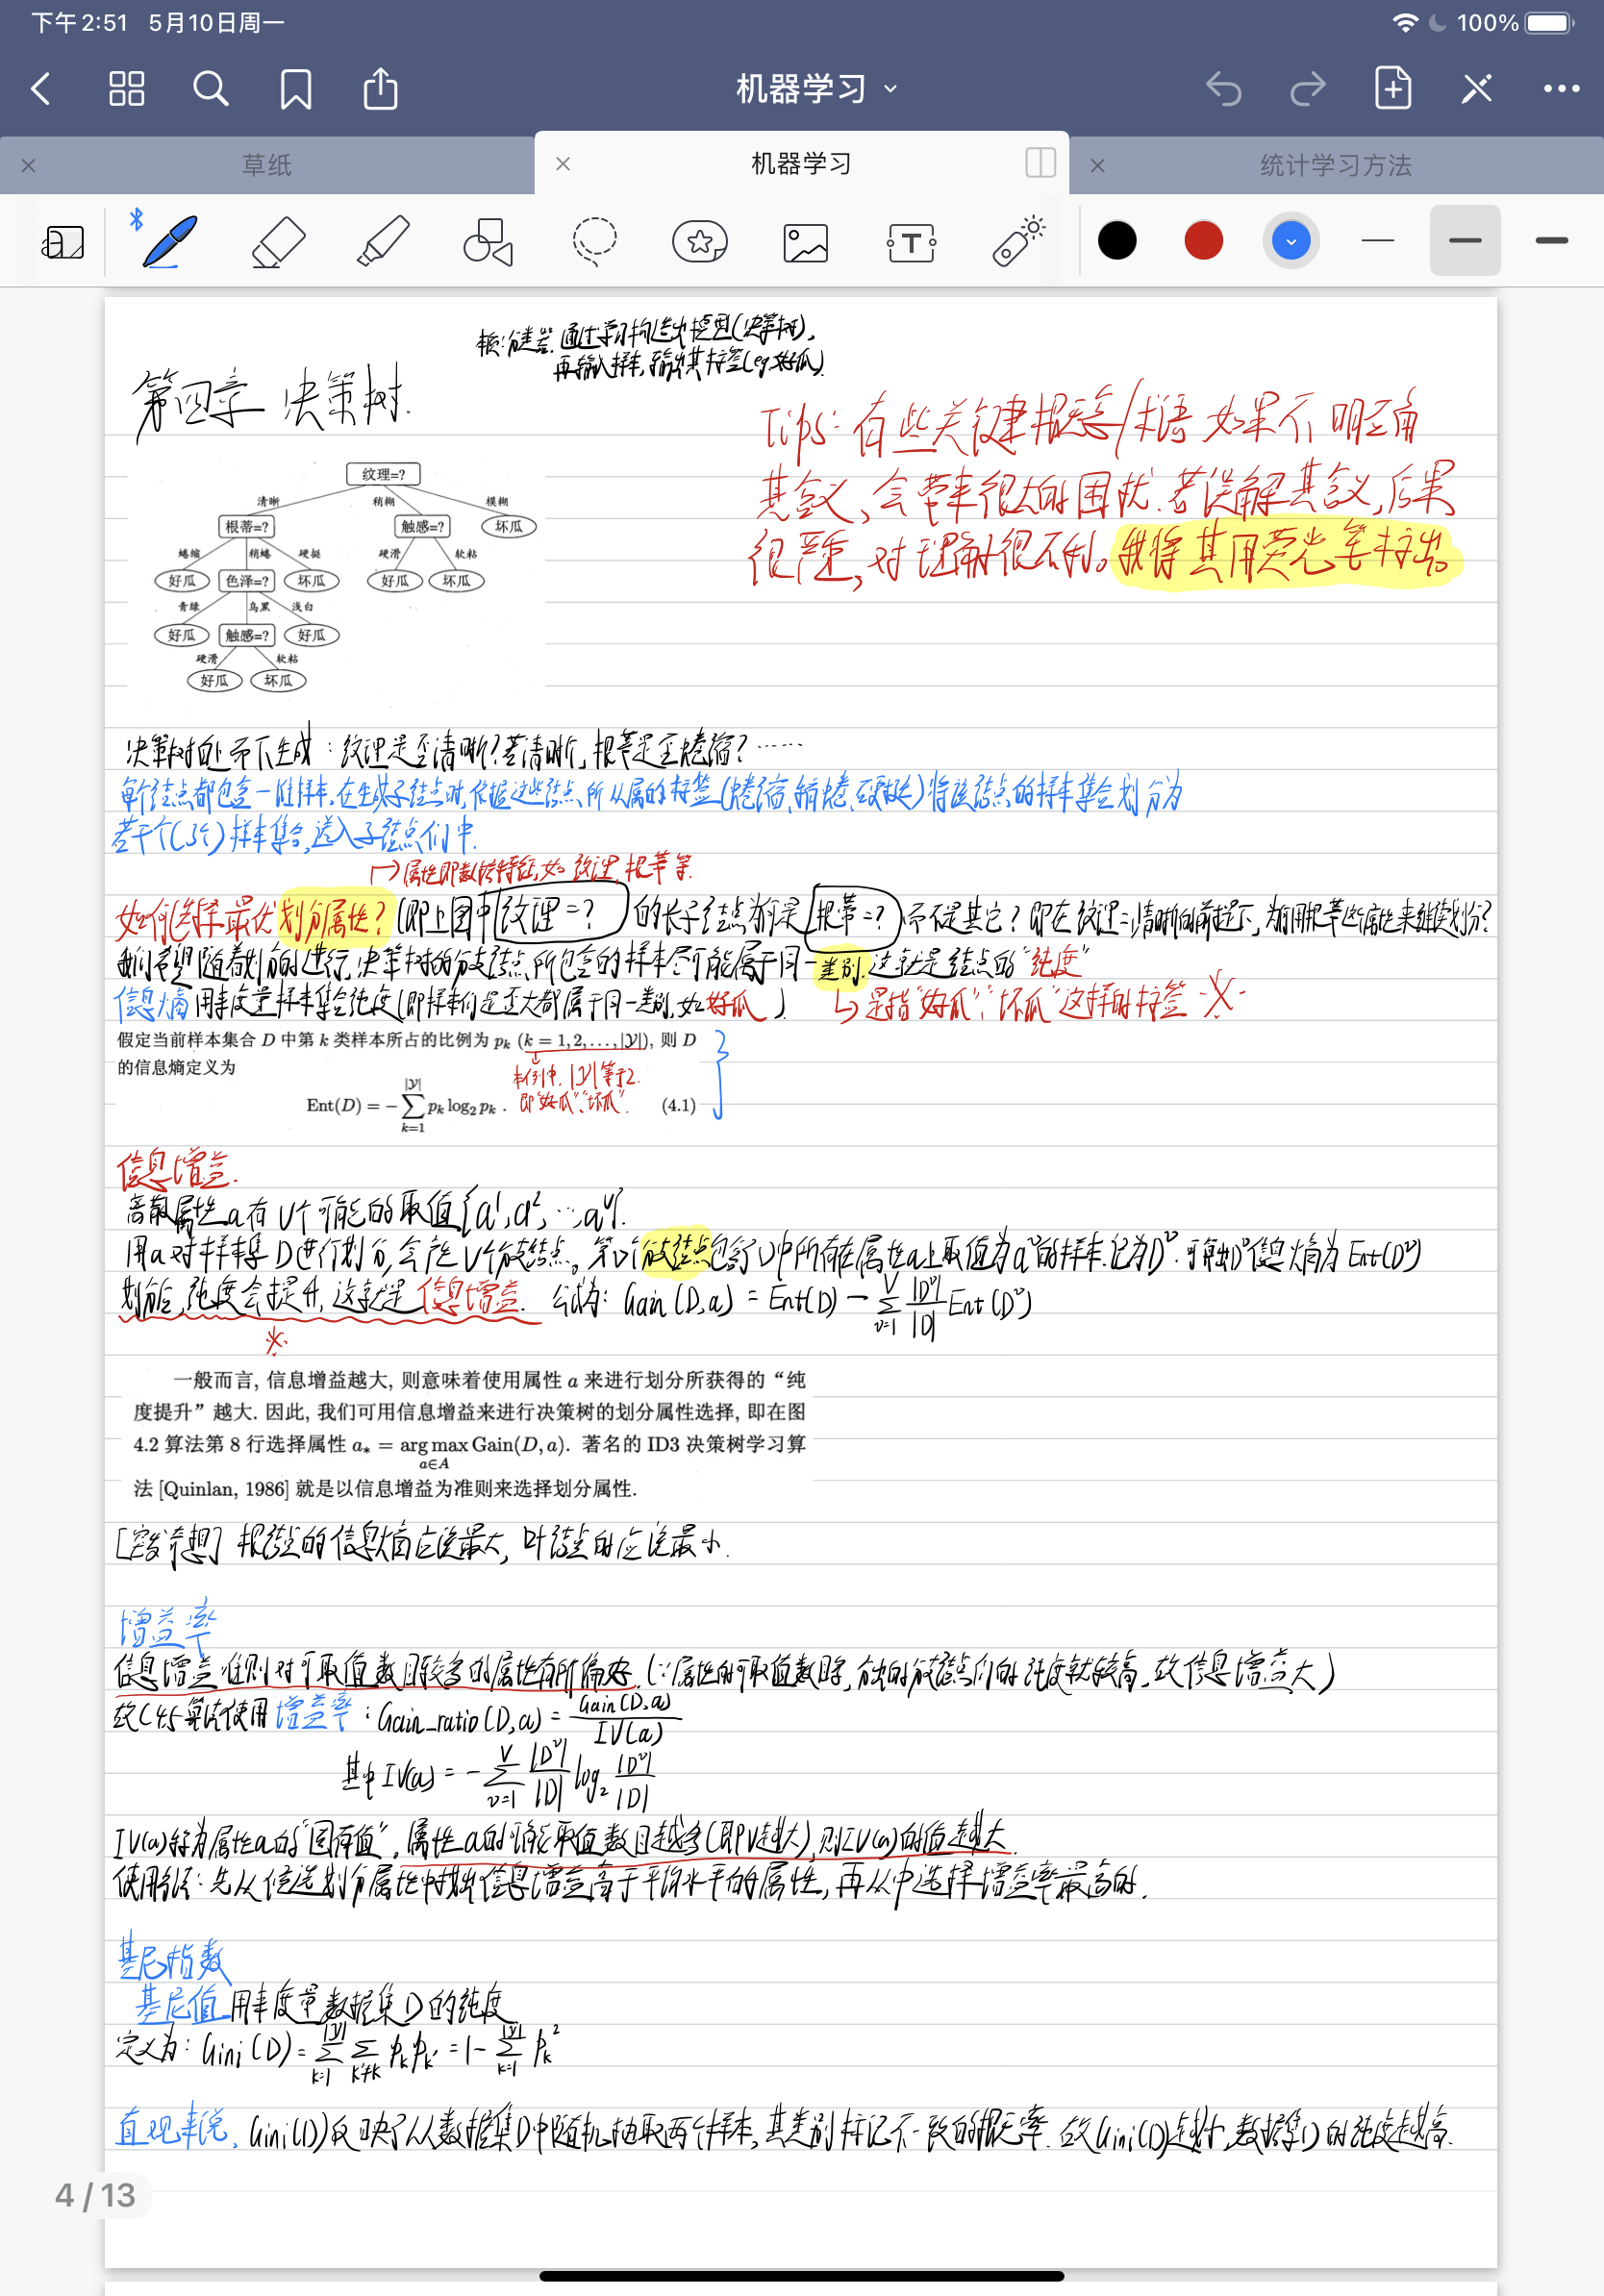
\includegraphics[scale=0.1]{./pic/12.eps}
 \end{figure}
\end{slide}

\begin{slide}{Ensemble Learning}
	Ensemble Learning:A decision tree is a prediction model used to predict the category of samples.In the structure of these trees, leaf nodes give categories and inner nodes represent attributes.
			\begin{figure}[htbp]
		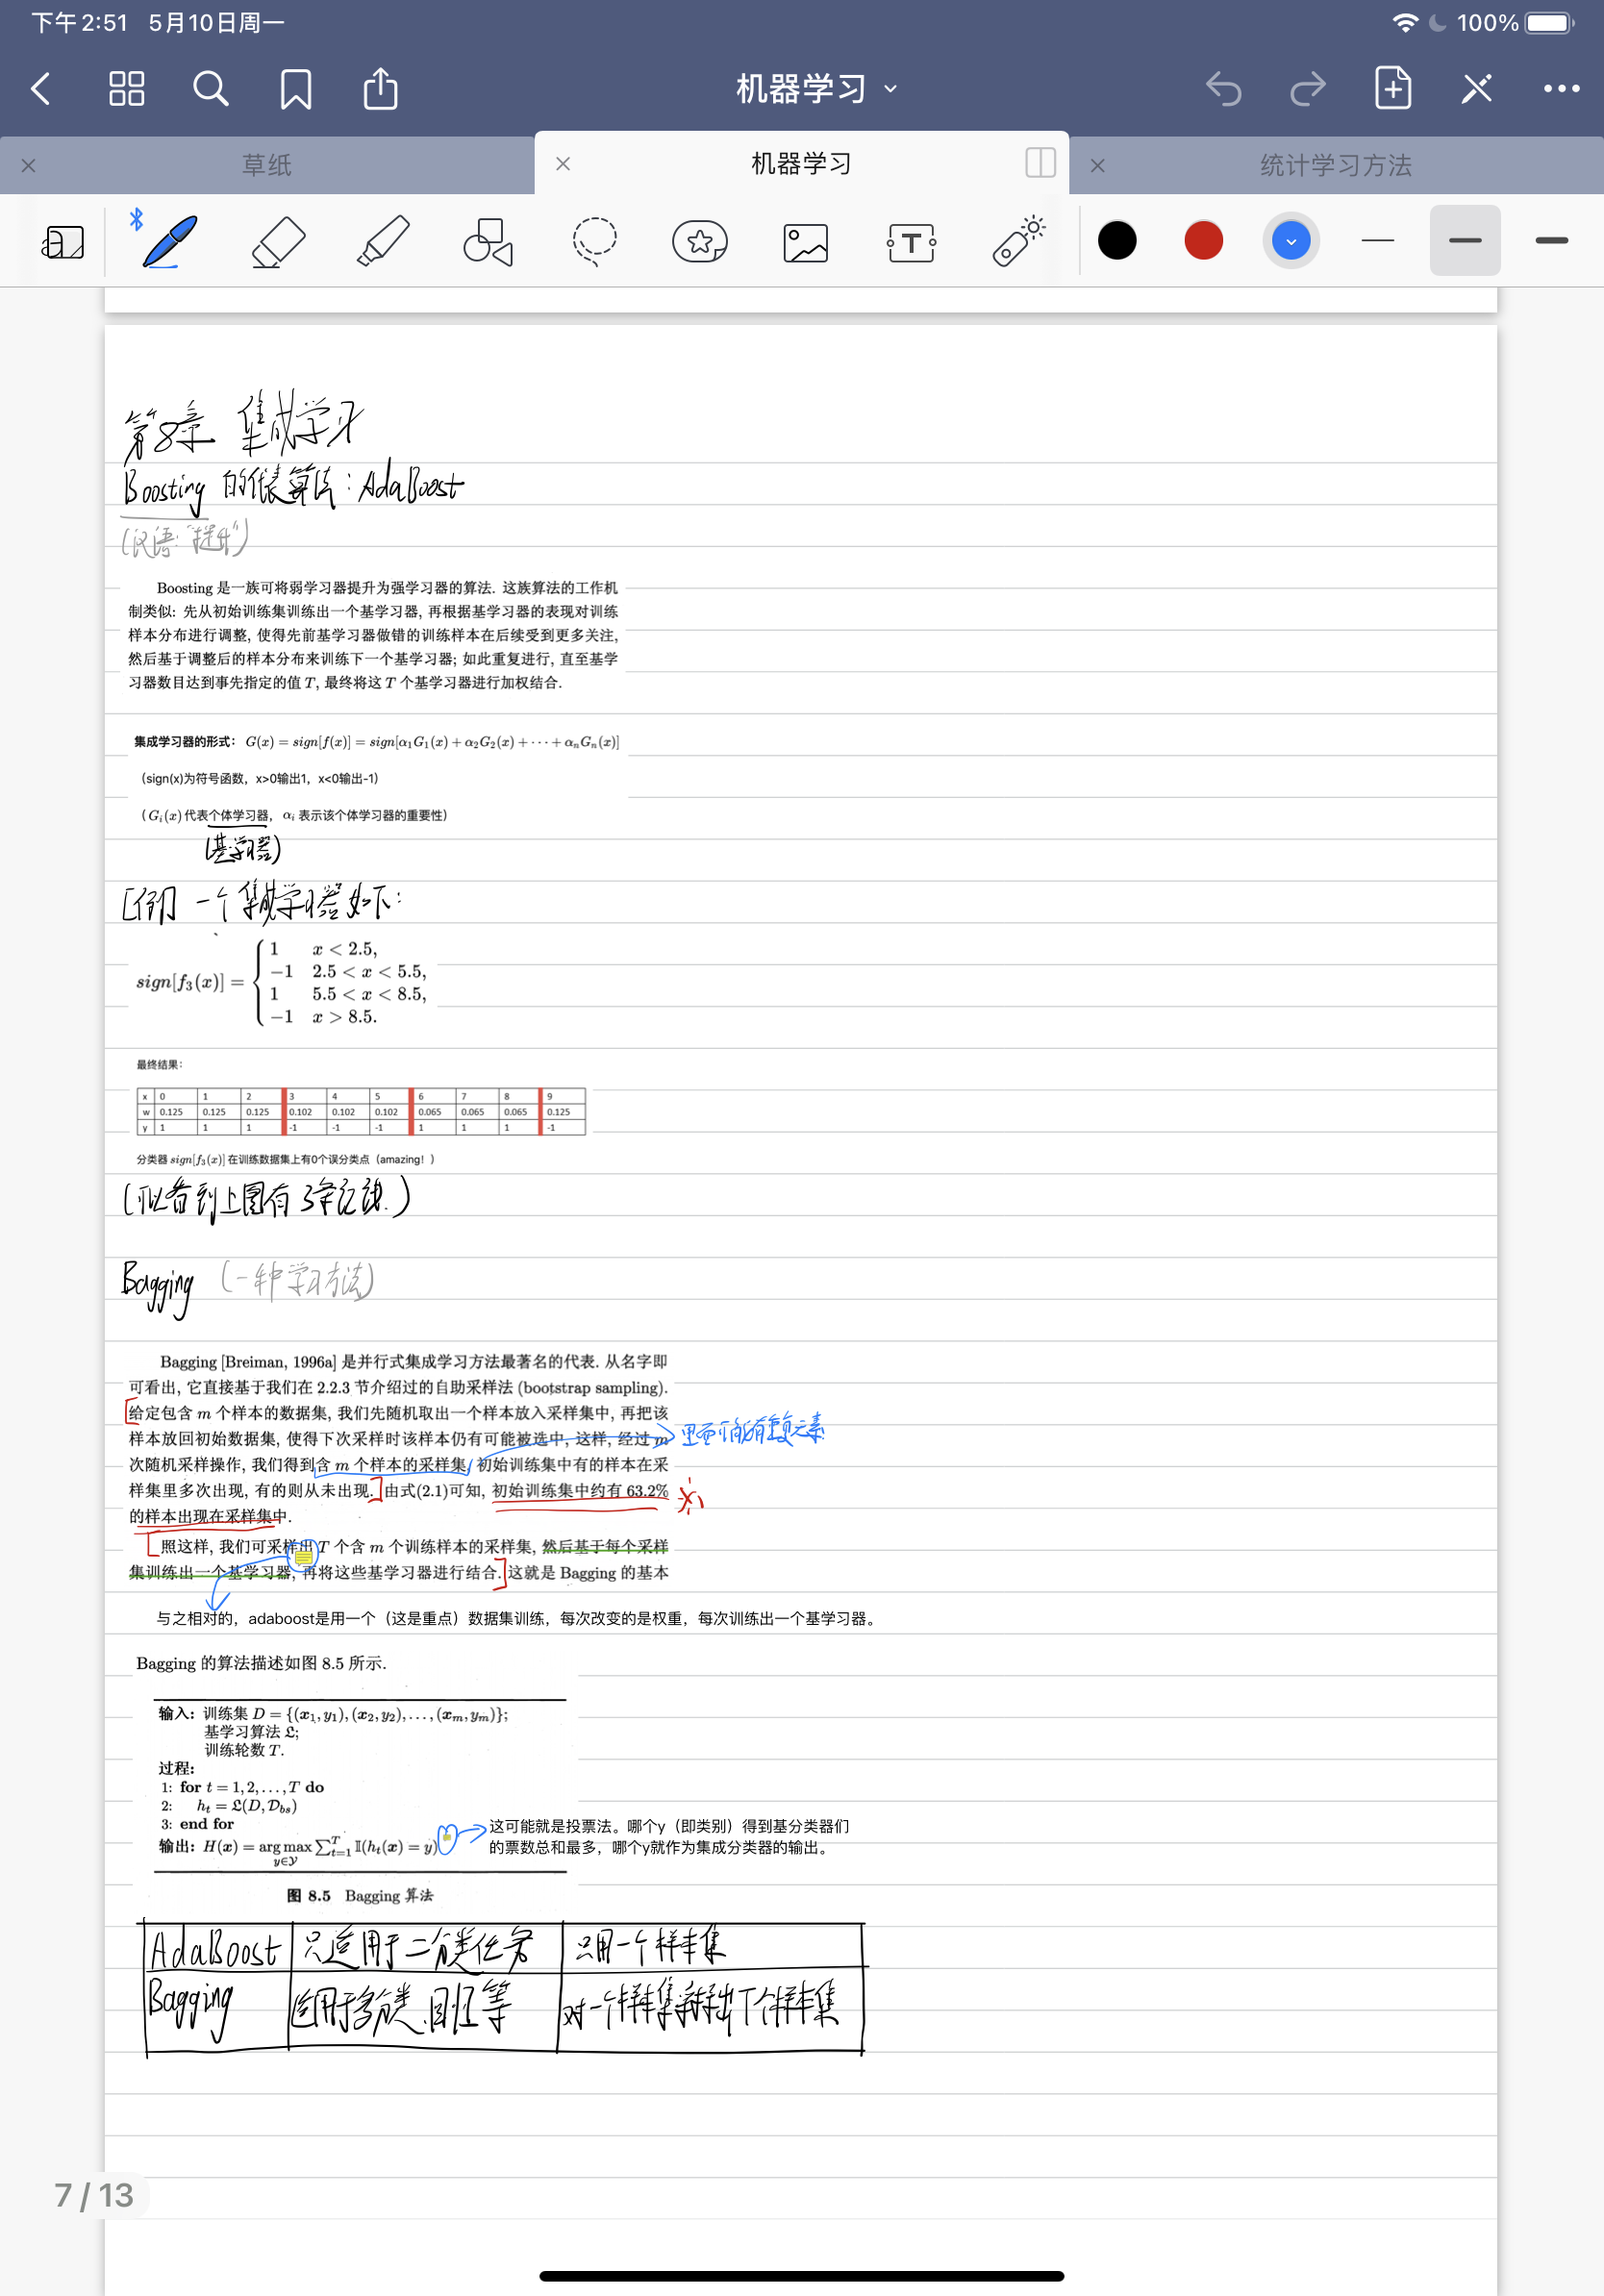
\includegraphics[scale=0.1]{./pic/13.eps}
	\end{figure}
\end{slide}

\begin{slide}{Neural Network}
	Neural Network:A mathematical or computational model that imitates the structure and function of a biological neural network and is used for estimating or approximating functions.
		\begin{figure}[htbp]
			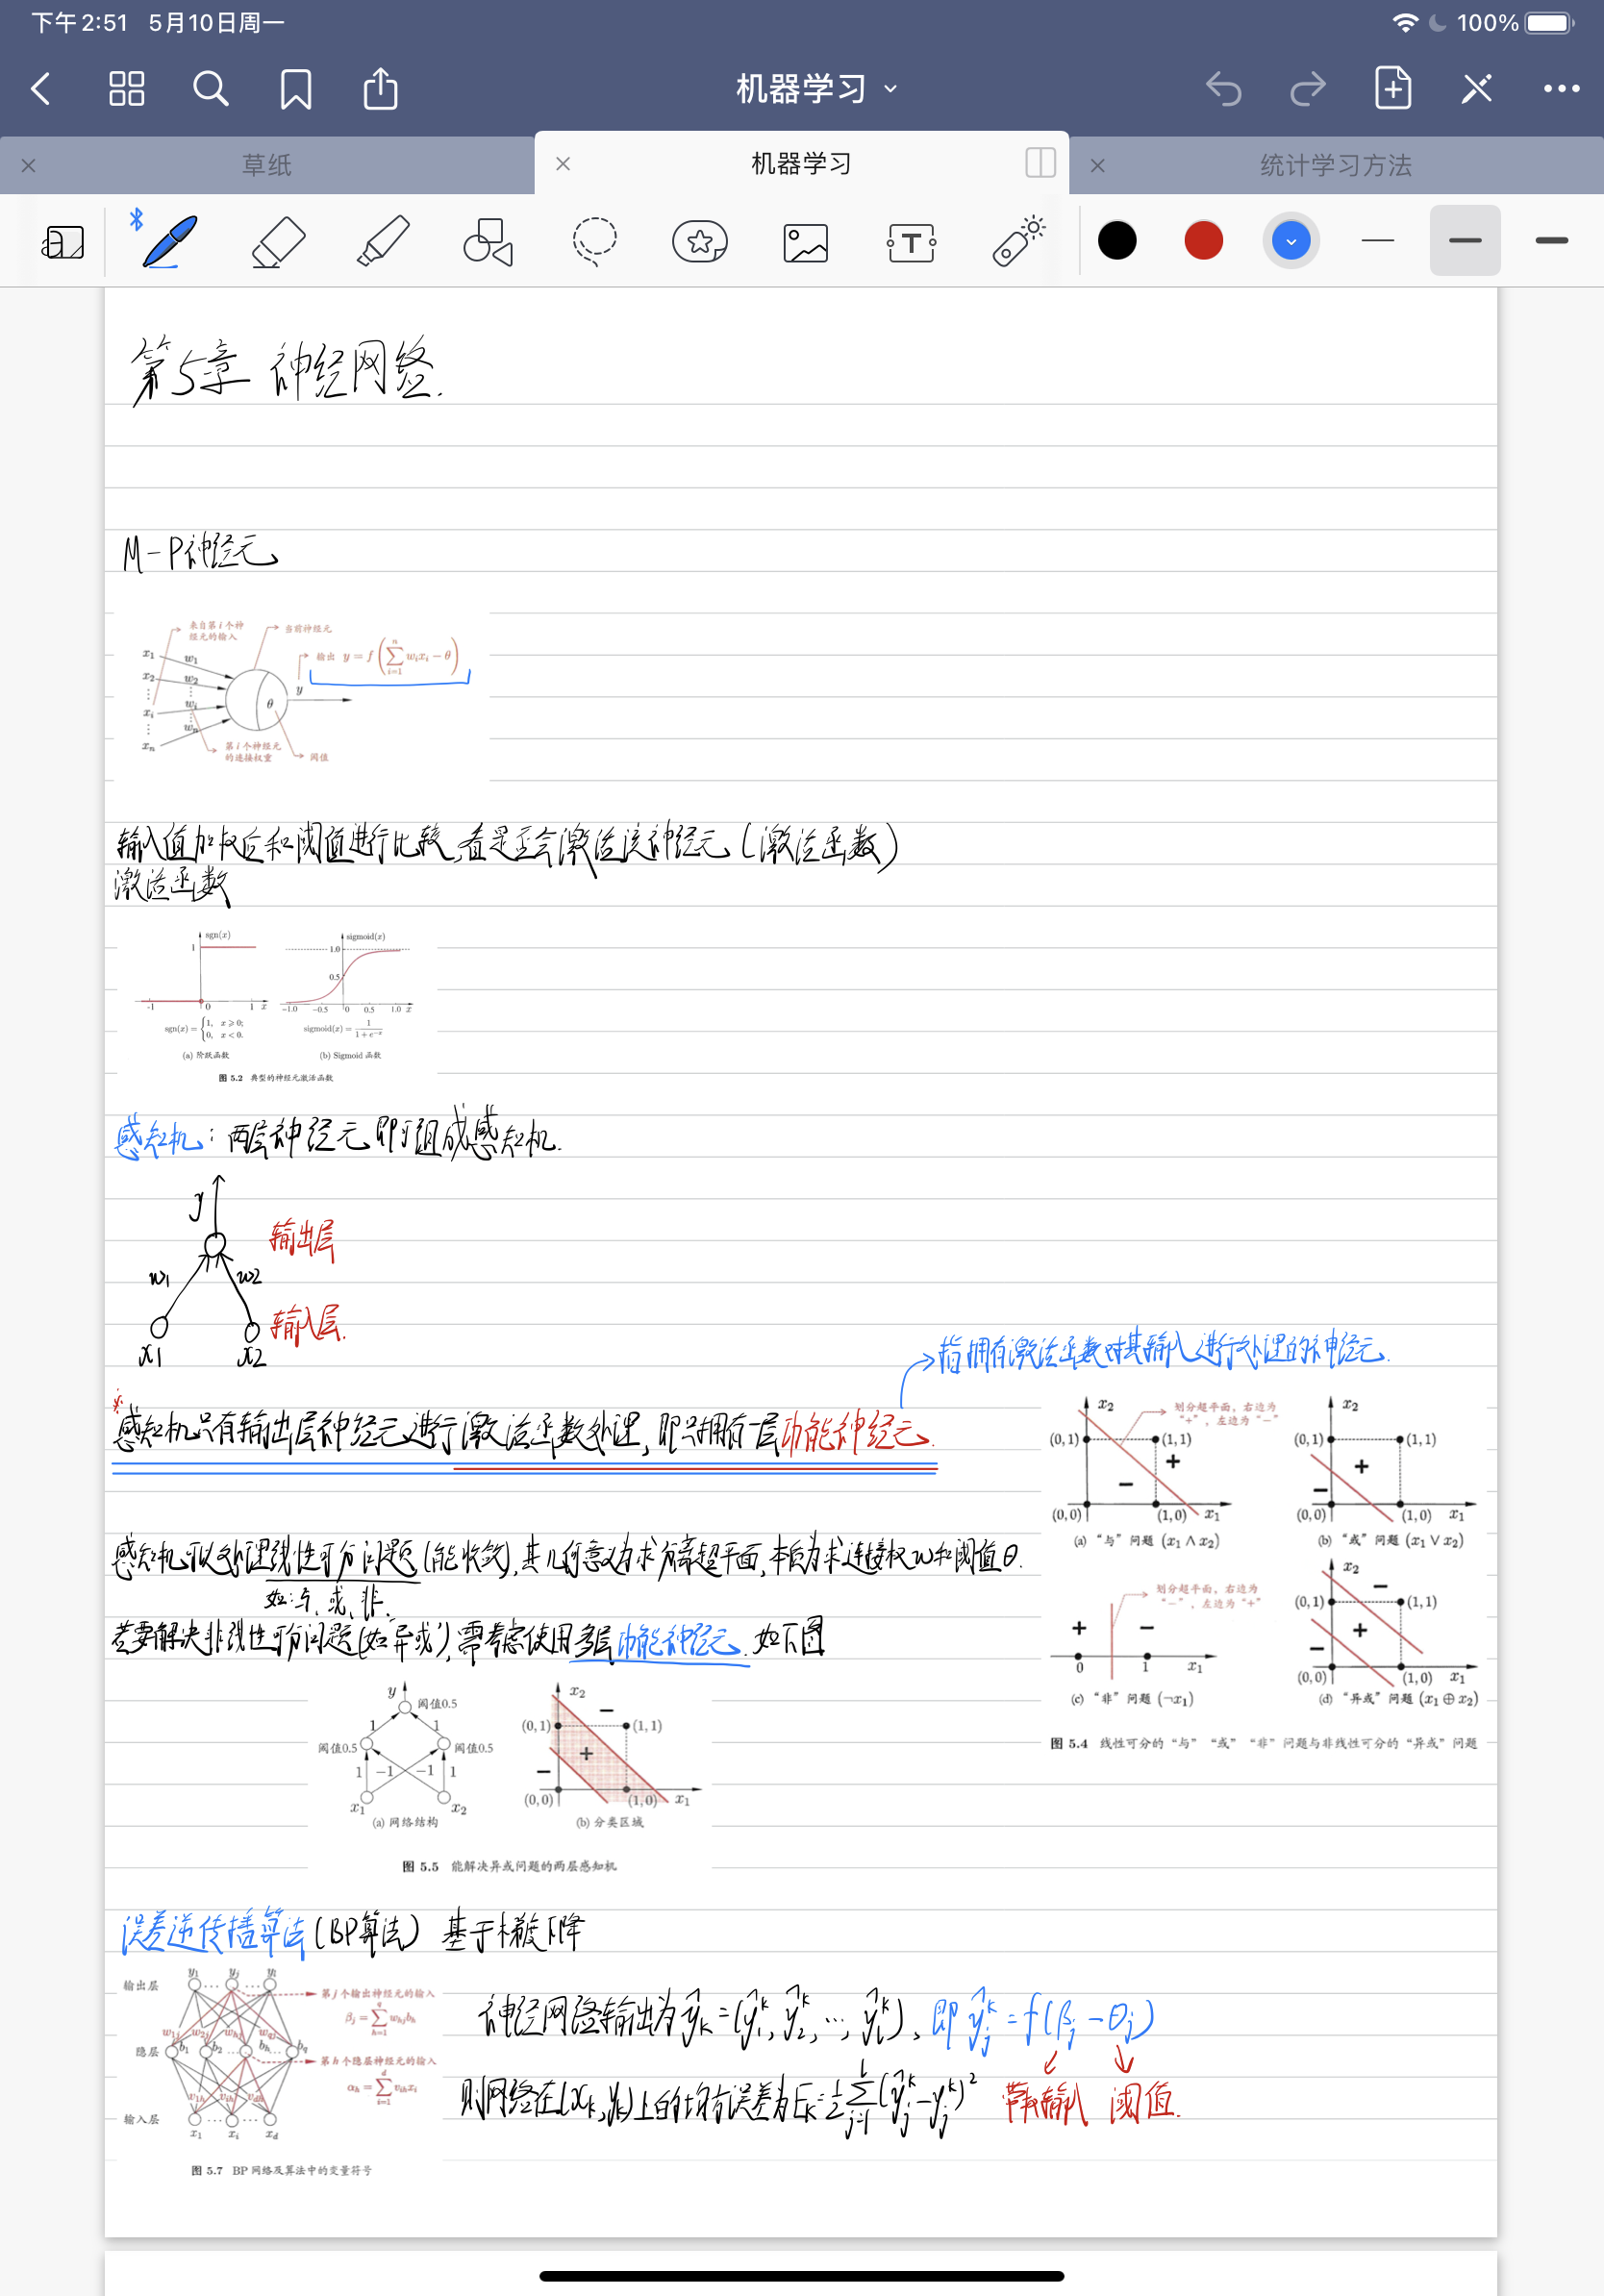
\includegraphics[scale=0.1]{./pic/11.eps}
		\end{figure}
\end{slide}
%%
%%==========================================================================================

%%==========================================================================================
%%


\section{Hands on practice}

%%
%%==========================================================================================


\begin{slide}{Generative Adversarial Network GAN}
	\begin{itemize}
	\item Generating Adversarial networks (GAN) is a method of unsupervised learning in which two neural networks play each other against each other.
	\end{itemize}

	\begin{center}
		\begin{figure}[htbp]
			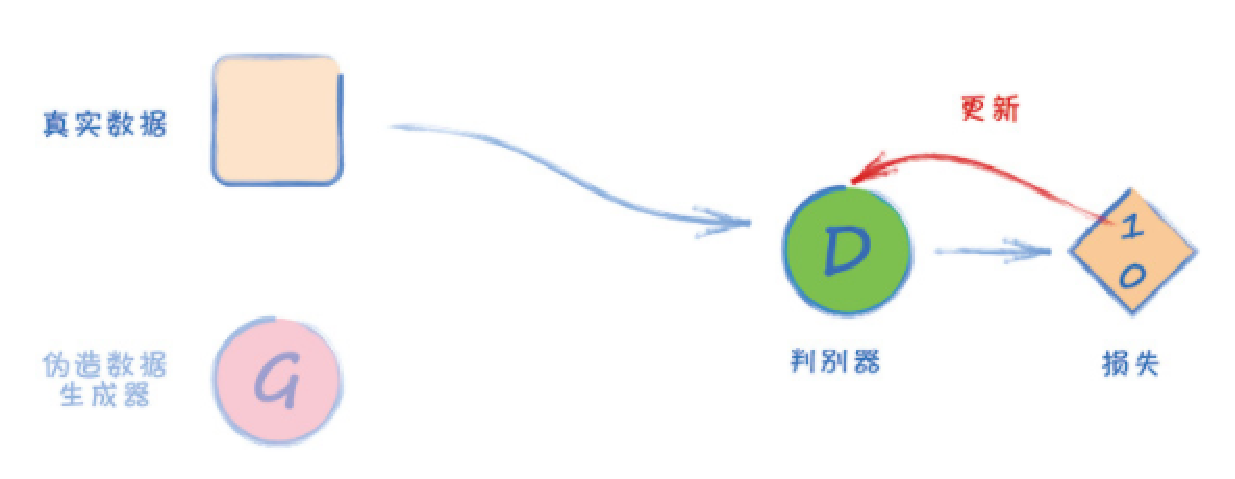
\includegraphics[scale=0.6]{./pic/14.eps}
			\caption{}
		\end{figure}
	\end{center}
	
\end{slide}

\begin{slide}[toc=,bm=]{Generative Adversarial Network GAN}
	
	\begin{center}
		\begin{figure}[htbp]
			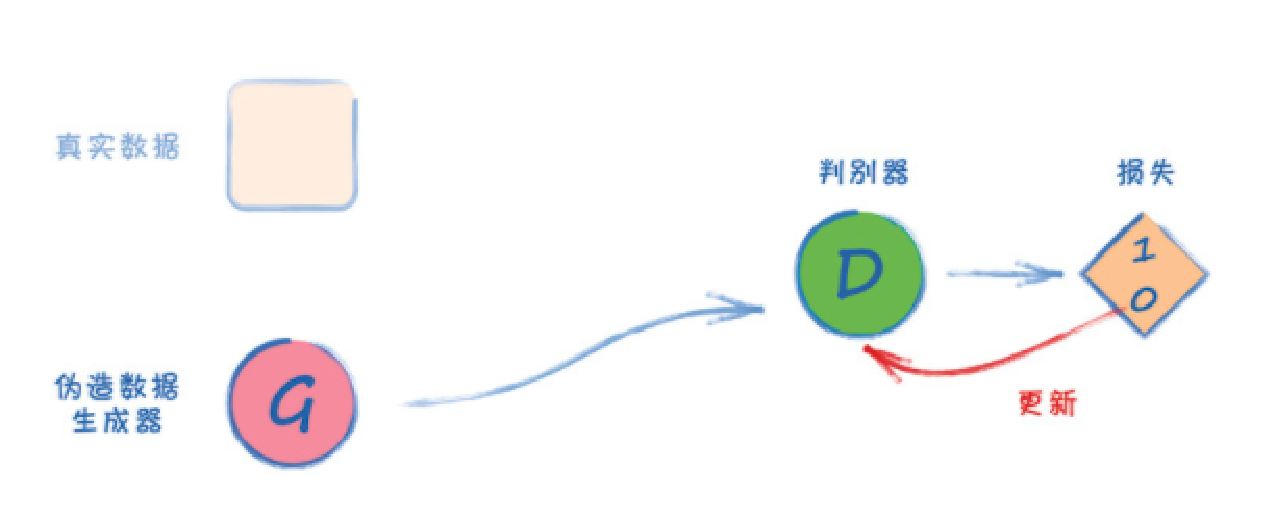
\includegraphics[scale=0.6]{./pic/15.eps}
			\caption{preview}
		\end{figure}
	\end{center}
	
\end{slide}

\begin{slide}[toc=,bm=]{Generative Adversarial Network GAN}
	
	\begin{center}
		\begin{figure}[htbp]
			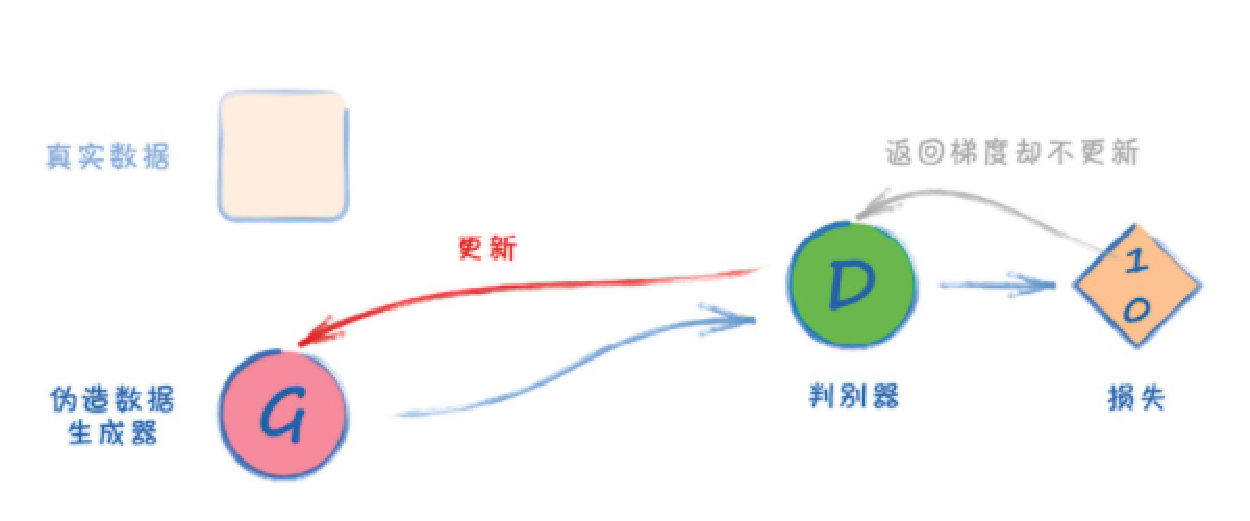
\includegraphics[scale=0.6]{./pic/16.eps}
			\caption{preview}
		\end{figure}
	\end{center}
	
\end{slide}



\section{Plan for the following week}

\begin{slide}{Plan for the following week}
	\begin{itemize}
	\item I'll continue to learn the basics next week.
	\item I'm going to go ahead and program this stuff out.
	\end{itemize}
\end{slide}


%%
%%==========================================================================================

%%==========================================================================================
%%

%%
%%==========================================================================================



%%
%%==========================================================================================


%%==========================================================================================
% TODO: Contact Page
\begin{wideslide}[toc=,bm=]{Contact Information}
\centering
\vspace{\stretch{1}}
\twocolumn[
lcolwidth=0.35\linewidth,
rcolwidth=0.65\linewidth
]
{
% \centerline{
\includegraphics[scale=.2]{tulip-logo.eps}}
}
{
\vspace{\stretch{1}}
Wang Mingxi\\
College of Computer Science and Technology\\
Jilin University, China
\begin{description}
 \item[\textcolor{orange}{\faEnvelope}] \href{mailto:mxwang@tulip.academy}
 {\textsc{\footnotesize{mxwang@tulip.academy}}}

 \item[\textcolor{orange}{\faHome}] \href{http://www.tulip.org.au}
 {\textsc{\footnotesize{Team for Universal Learning and Intelligent Processing}}}
\end{description}
}
\vspace{\stretch{1}}
\end{wideslide}

\end{document}

\endinput
